\scanpage{27}
\mspage{18}
% archive sheet number: 27

% source lines 1--6
 i.e. des \deleted{figures} parties $F\subset M$ telles que
\[
\begin{aligned}
\text{a)}\quad &F\text{ fermé pour }\leq\\
\text{b)}\quad &X,Y\in F\ \Longrightarrow\ X\unsure{\gtrless|\lessgtr}_{\unsure{\mathrm{pol}|\mathrm{pré}}}Y,\quad\text{i.e.}\quad
\left\{\begin{aligned}
&\text{1°)}\ X'\in\deleted{\widetilde X}\widetilde X\cap\widetilde Y,\ Y'\in\deleted{\widetilde X}\widetilde X\cap\widetilde Y\\
&\hspace{2em}\Longrightarrow X'\unsure{|0|\,|\,|\circ|}Y'\\
&\text{2°)}\ \forall X'\in\widetilde X,\ Y'\in\widetilde Y,\ \widetilde X\cap\widetilde Y\\
&\text{est vide ou a un}\\
&\text{plus grand élément.}
\end{aligned}\right.
\end{aligned}
\]

\deleted{Ceci posé, on trouve}

% source lines 7--10
\uline{NB} Même si $M$ est polyédral, on aura en général une inclusion \uline{stricte} $\mathrm{Fig}_{\mathrm{pol}}(M)\subsetneq\mathrm{Fig}(M)$.

\figure{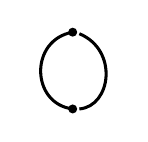
\begin{tikzpicture}[scale=.65]
\draw[line width=1.1pt] (0,.75) .. controls (-.85,.6) and (-.82,-.65) .. (0,-.75);
\draw[line width=1.1pt] (.13,.72) .. controls (.9,.4) and (.75,-.7) .. (.13,-.75);
\fill (0,.75) circle (2.5pt);\fill (0,-.75) circle (2.5pt);
\end{tikzpicture}}
Cette figure circulaire est dans $\mathrm{Fig}(M)$, mais non dans $\mathrm{Fig}_{\mathrm{pol}}(M)$, pour $M$ magasin polyédral \unsure{convenable}.

% left margin, with two drawings
\margin{Exemple analogue avec $X\ll Y$ mais non $X\ll_{\mathrm{pol}}Y$ (\unsure{à l'intérieur des} \unsure{2-simplexes|2-simples})}
\figure{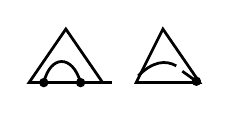
\begin{tikzpicture}[scale=.85]
\draw[line width=1pt] (0,0)--(.55,.8)--(1.1,0)--cycle;
\draw[line width=1pt] (.22,0) .. controls (.32,.42) and (.65,.42) .. (.77,0);
\fill (.22,0) circle (2pt);\draw[line width=1pt] (1.1,0)--(1.24,0);\fill (.77,0) circle (2pt);
\draw[line width=1pt] (1.6,0)--(2,.8)--(2.55,0)--cycle;
\draw[line width=1pt] (1.63,.1) .. controls (1.85,.32) and (2.04,.34) .. (2.2,.25);
\draw[line width=1pt] (2.29,.17)--(2.5,.02);
\fill (2.5,.02) circle (2pt);
\end{tikzpicture}}

% source lines 11--18
\uline{Scholie} Les propriétés \inserted{algébriques} formelles de $\unsure{\mathcal F|F}=\mathrm{Fig}_{\mathrm{pol}}(M)$, muni des $\leq,\ll_{\mathrm{pol}},\gtrless_{\mathrm{pol}}$, et ses relations avec $M$ (muni des relations induites) seront sensiblement les mêmes que pour $\leq,\ll_{\deleted{\mathrm{pol}}},\gtrless_{\deleted{\mathrm{pol}}}$. \deleted{\unsure{et}} La seule différence est dans l'explicitation de $\gtrless_{\mathrm{pol}}$ \unsure{resp.} $\gtrless$, en termes de la relation de disjonction interne $|0|$.

On devrait passer en revue \deleted{toutes} les propositions pertinentes\ldots

Je signale seulement celle-ci

% source lines 19--24
\uline{Prop} Si $F,G\in\mathrm{Fig}_{\mathrm{pol}}$, alors \deleted{$\{F,G\}$ \unsure{majoré}} conditions équivalentes
\[
\begin{aligned}
\text{(i)}\quad &\{F,G\}\text{ majoré pour }\leq\\
\text{(ii)}\quad &\mathrm{Sup}^{\leq}(F,G)\text{ existe}\\
\text{(iii)}\quad &F\cup G\text{ (réunion dans }\unsure{\mathcal P|\mathscr P}(M)\text{)}\in\mathrm{Fig}_{\mathrm{pol}}(M)\\
\text{(iv)}\quad &\forall X\in\widetilde F,\ Y\in\widetilde G,\text{ on a }X\gtrless_{\mathrm{pol}}Y.
\end{aligned}
\]
\margin{On écrit alors $F\gtrless_{\mathrm{pol}}G$}

% source lines 25--29
Dans certains contextes, on laissera tomber l'indice pol à $\gtrless$, $\ll$, quand il est bien entendu qu'il ne s'agit que des relations ``polyédrales''.

\uline{Atelier polyédral} Se définit essentiellement \inserted{(en termes d'un \unsure{magasin} polyédral $M$ et de $\mathrm{Fig}_{\mathrm{pol}}(M)$,)}
